\documentclass{article}
\usepackage{iclr2027_conference,times}
%%%%% NEW MATH DEFINITIONS %%%%%

\usepackage{amsmath,amsfonts,bm}

% Mark sections of captions for referring to divisions of figures
\newcommand{\figleft}{{\em (Left)}}
\newcommand{\figcenter}{{\em (Center)}}
\newcommand{\figright}{{\em (Right)}}
\newcommand{\figtop}{{\em (Top)}}
\newcommand{\figbottom}{{\em (Bottom)}}
\newcommand{\captiona}{{\em (a)}}
\newcommand{\captionb}{{\em (b)}}
\newcommand{\captionc}{{\em (c)}}
\newcommand{\captiond}{{\em (d)}}

% Highlight a newly defined term
\newcommand{\newterm}[1]{{\bf #1}}


% Figure reference, lower-case.
\def\figref#1{figure~\ref{#1}}
% Figure reference, capital. For start of sentence
\def\Figref#1{Figure~\ref{#1}}
\def\twofigref#1#2{figures \ref{#1} and \ref{#2}}
\def\quadfigref#1#2#3#4{figures \ref{#1}, \ref{#2}, \ref{#3} and \ref{#4}}
% Section reference, lower-case.
\def\secref#1{section~\ref{#1}}
% Section reference, capital.
\def\Secref#1{Section~\ref{#1}}
% Reference to two sections.
\def\twosecrefs#1#2{sections \ref{#1} and \ref{#2}}
% Reference to three sections.
\def\secrefs#1#2#3{sections \ref{#1}, \ref{#2} and \ref{#3}}
% Reference to an equation, lower-case.
\def\eqref#1{equation~\ref{#1}}
% Reference to an equation, upper case
\def\Eqref#1{Equation~\ref{#1}}
% A raw reference to an equation---avoid using if possible
\def\plaineqref#1{\ref{#1}}
% Reference to a chapter, lower-case.
\def\chapref#1{chapter~\ref{#1}}
% Reference to an equation, upper case.
\def\Chapref#1{Chapter~\ref{#1}}
% Reference to a range of chapters
\def\rangechapref#1#2{chapters\ref{#1}--\ref{#2}}
% Reference to an algorithm, lower-case.
\def\algref#1{algorithm~\ref{#1}}
% Reference to an algorithm, upper case.
\def\Algref#1{Algorithm~\ref{#1}}
\def\twoalgref#1#2{algorithms \ref{#1} and \ref{#2}}
\def\Twoalgref#1#2{Algorithms \ref{#1} and \ref{#2}}
% Reference to a part, lower case
\def\partref#1{part~\ref{#1}}
% Reference to a part, upper case
\def\Partref#1{Part~\ref{#1}}
\def\twopartref#1#2{parts \ref{#1} and \ref{#2}}

\def\ceil#1{\lceil #1 \rceil}
\def\floor#1{\lfloor #1 \rfloor}
\def\1{\bm{1}}
\newcommand{\train}{\mathcal{D}}
\newcommand{\valid}{\mathcal{D_{\mathrm{valid}}}}
\newcommand{\test}{\mathcal{D_{\mathrm{test}}}}

\def\eps{{\epsilon}}


% Random variables
\def\reta{{\textnormal{$\eta$}}}
\def\ra{{\textnormal{a}}}
\def\rb{{\textnormal{b}}}
\def\rc{{\textnormal{c}}}
\def\rd{{\textnormal{d}}}
\def\re{{\textnormal{e}}}
\def\rf{{\textnormal{f}}}
\def\rg{{\textnormal{g}}}
\def\rh{{\textnormal{h}}}
\def\ri{{\textnormal{i}}}
\def\rj{{\textnormal{j}}}
\def\rk{{\textnormal{k}}}
\def\rl{{\textnormal{l}}}
% rm is already a command, just don't name any random variables m
\def\rn{{\textnormal{n}}}
\def\ro{{\textnormal{o}}}
\def\rp{{\textnormal{p}}}
\def\rq{{\textnormal{q}}}
\def\rr{{\textnormal{r}}}
\def\rs{{\textnormal{s}}}
\def\rt{{\textnormal{t}}}
\def\ru{{\textnormal{u}}}
\def\rv{{\textnormal{v}}}
\def\rw{{\textnormal{w}}}
\def\rx{{\textnormal{x}}}
\def\ry{{\textnormal{y}}}
\def\rz{{\textnormal{z}}}

% Random vectors
\def\rvepsilon{{\mathbf{\epsilon}}}
\def\rvtheta{{\mathbf{\theta}}}
\def\rva{{\mathbf{a}}}
\def\rvb{{\mathbf{b}}}
\def\rvc{{\mathbf{c}}}
\def\rvd{{\mathbf{d}}}
\def\rve{{\mathbf{e}}}
\def\rvf{{\mathbf{f}}}
\def\rvg{{\mathbf{g}}}
\def\rvh{{\mathbf{h}}}
\def\rvu{{\mathbf{i}}}
\def\rvj{{\mathbf{j}}}
\def\rvk{{\mathbf{k}}}
\def\rvl{{\mathbf{l}}}
\def\rvm{{\mathbf{m}}}
\def\rvn{{\mathbf{n}}}
\def\rvo{{\mathbf{o}}}
\def\rvp{{\mathbf{p}}}
\def\rvq{{\mathbf{q}}}
\def\rvr{{\mathbf{r}}}
\def\rvs{{\mathbf{s}}}
\def\rvt{{\mathbf{t}}}
\def\rvu{{\mathbf{u}}}
\def\rvv{{\mathbf{v}}}
\def\rvw{{\mathbf{w}}}
\def\rvx{{\mathbf{x}}}
\def\rvy{{\mathbf{y}}}
\def\rvz{{\mathbf{z}}}

% Elements of random vectors
\def\erva{{\textnormal{a}}}
\def\ervb{{\textnormal{b}}}
\def\ervc{{\textnormal{c}}}
\def\ervd{{\textnormal{d}}}
\def\erve{{\textnormal{e}}}
\def\ervf{{\textnormal{f}}}
\def\ervg{{\textnormal{g}}}
\def\ervh{{\textnormal{h}}}
\def\ervi{{\textnormal{i}}}
\def\ervj{{\textnormal{j}}}
\def\ervk{{\textnormal{k}}}
\def\ervl{{\textnormal{l}}}
\def\ervm{{\textnormal{m}}}
\def\ervn{{\textnormal{n}}}
\def\ervo{{\textnormal{o}}}
\def\ervp{{\textnormal{p}}}
\def\ervq{{\textnormal{q}}}
\def\ervr{{\textnormal{r}}}
\def\ervs{{\textnormal{s}}}
\def\ervt{{\textnormal{t}}}
\def\ervu{{\textnormal{u}}}
\def\ervv{{\textnormal{v}}}
\def\ervw{{\textnormal{w}}}
\def\ervx{{\textnormal{x}}}
\def\ervy{{\textnormal{y}}}
\def\ervz{{\textnormal{z}}}

% Random matrices
\def\rmA{{\mathbf{A}}}
\def\rmB{{\mathbf{B}}}
\def\rmC{{\mathbf{C}}}
\def\rmD{{\mathbf{D}}}
\def\rmE{{\mathbf{E}}}
\def\rmF{{\mathbf{F}}}
\def\rmG{{\mathbf{G}}}
\def\rmH{{\mathbf{H}}}
\def\rmI{{\mathbf{I}}}
\def\rmJ{{\mathbf{J}}}
\def\rmK{{\mathbf{K}}}
\def\rmL{{\mathbf{L}}}
\def\rmM{{\mathbf{M}}}
\def\rmN{{\mathbf{N}}}
\def\rmO{{\mathbf{O}}}
\def\rmP{{\mathbf{P}}}
\def\rmQ{{\mathbf{Q}}}
\def\rmR{{\mathbf{R}}}
\def\rmS{{\mathbf{S}}}
\def\rmT{{\mathbf{T}}}
\def\rmU{{\mathbf{U}}}
\def\rmV{{\mathbf{V}}}
\def\rmW{{\mathbf{W}}}
\def\rmX{{\mathbf{X}}}
\def\rmY{{\mathbf{Y}}}
\def\rmZ{{\mathbf{Z}}}

% Elements of random matrices
\def\ermA{{\textnormal{A}}}
\def\ermB{{\textnormal{B}}}
\def\ermC{{\textnormal{C}}}
\def\ermD{{\textnormal{D}}}
\def\ermE{{\textnormal{E}}}
\def\ermF{{\textnormal{F}}}
\def\ermG{{\textnormal{G}}}
\def\ermH{{\textnormal{H}}}
\def\ermI{{\textnormal{I}}}
\def\ermJ{{\textnormal{J}}}
\def\ermK{{\textnormal{K}}}
\def\ermL{{\textnormal{L}}}
\def\ermM{{\textnormal{M}}}
\def\ermN{{\textnormal{N}}}
\def\ermO{{\textnormal{O}}}
\def\ermP{{\textnormal{P}}}
\def\ermQ{{\textnormal{Q}}}
\def\ermR{{\textnormal{R}}}
\def\ermS{{\textnormal{S}}}
\def\ermT{{\textnormal{T}}}
\def\ermU{{\textnormal{U}}}
\def\ermV{{\textnormal{V}}}
\def\ermW{{\textnormal{W}}}
\def\ermX{{\textnormal{X}}}
\def\ermY{{\textnormal{Y}}}
\def\ermZ{{\textnormal{Z}}}

% Vectors
\def\vzero{{\bm{0}}}
\def\vone{{\bm{1}}}
\def\vmu{{\bm{\mu}}}
\def\vtheta{{\bm{\theta}}}
\def\va{{\bm{a}}}
\def\vb{{\bm{b}}}
\def\vc{{\bm{c}}}
\def\vd{{\bm{d}}}
\def\ve{{\bm{e}}}
\def\vf{{\bm{f}}}
\def\vg{{\bm{g}}}
\def\vh{{\bm{h}}}
\def\vi{{\bm{i}}}
\def\vj{{\bm{j}}}
\def\vk{{\bm{k}}}
\def\vl{{\bm{l}}}
\def\vm{{\bm{m}}}
\def\vn{{\bm{n}}}
\def\vo{{\bm{o}}}
\def\vp{{\bm{p}}}
\def\vq{{\bm{q}}}
\def\vr{{\bm{r}}}
\def\vs{{\bm{s}}}
\def\vt{{\bm{t}}}
\def\vu{{\bm{u}}}
\def\vv{{\bm{v}}}
\def\vw{{\bm{w}}}
\def\vx{{\bm{x}}}
\def\vy{{\bm{y}}}
\def\vz{{\bm{z}}}

% Elements of vectors
\def\evalpha{{\alpha}}
\def\evbeta{{\beta}}
\def\evepsilon{{\epsilon}}
\def\evlambda{{\lambda}}
\def\evomega{{\omega}}
\def\evmu{{\mu}}
\def\evpsi{{\psi}}
\def\evsigma{{\sigma}}
\def\evtheta{{\theta}}
\def\eva{{a}}
\def\evb{{b}}
\def\evc{{c}}
\def\evd{{d}}
\def\eve{{e}}
\def\evf{{f}}
\def\evg{{g}}
\def\evh{{h}}
\def\evi{{i}}
\def\evj{{j}}
\def\evk{{k}}
\def\evl{{l}}
\def\evm{{m}}
\def\evn{{n}}
\def\evo{{o}}
\def\evp{{p}}
\def\evq{{q}}
\def\evr{{r}}
\def\evs{{s}}
\def\evt{{t}}
\def\evu{{u}}
\def\evv{{v}}
\def\evw{{w}}
\def\evx{{x}}
\def\evy{{y}}
\def\evz{{z}}

% Matrix
\def\mA{{\bm{A}}}
\def\mB{{\bm{B}}}
\def\mC{{\bm{C}}}
\def\mD{{\bm{D}}}
\def\mE{{\bm{E}}}
\def\mF{{\bm{F}}}
\def\mG{{\bm{G}}}
\def\mH{{\bm{H}}}
\def\mI{{\bm{I}}}
\def\mJ{{\bm{J}}}
\def\mK{{\bm{K}}}
\def\mL{{\bm{L}}}
\def\mM{{\bm{M}}}
\def\mN{{\bm{N}}}
\def\mO{{\bm{O}}}
\def\mP{{\bm{P}}}
\def\mQ{{\bm{Q}}}
\def\mR{{\bm{R}}}
\def\mS{{\bm{S}}}
\def\mT{{\bm{T}}}
\def\mU{{\bm{U}}}
\def\mV{{\bm{V}}}
\def\mW{{\bm{W}}}
\def\mX{{\bm{X}}}
\def\mY{{\bm{Y}}}
\def\mZ{{\bm{Z}}}
\def\mBeta{{\bm{\beta}}}
\def\mPhi{{\bm{\Phi}}}
\def\mLambda{{\bm{\Lambda}}}
\def\mSigma{{\bm{\Sigma}}}

% Tensor
\DeclareMathAlphabet{\mathsfit}{\encodingdefault}{\sfdefault}{m}{sl}
\SetMathAlphabet{\mathsfit}{bold}{\encodingdefault}{\sfdefault}{bx}{n}
\newcommand{\tens}[1]{\bm{\mathsfit{#1}}}
\def\tA{{\tens{A}}}
\def\tB{{\tens{B}}}
\def\tC{{\tens{C}}}
\def\tD{{\tens{D}}}
\def\tE{{\tens{E}}}
\def\tF{{\tens{F}}}
\def\tG{{\tens{G}}}
\def\tH{{\tens{H}}}
\def\tI{{\tens{I}}}
\def\tJ{{\tens{J}}}
\def\tK{{\tens{K}}}
\def\tL{{\tens{L}}}
\def\tM{{\tens{M}}}
\def\tN{{\tens{N}}}
\def\tO{{\tens{O}}}
\def\tP{{\tens{P}}}
\def\tQ{{\tens{Q}}}
\def\tR{{\tens{R}}}
\def\tS{{\tens{S}}}
\def\tT{{\tens{T}}}
\def\tU{{\tens{U}}}
\def\tV{{\tens{V}}}
\def\tW{{\tens{W}}}
\def\tX{{\tens{X}}}
\def\tY{{\tens{Y}}}
\def\tZ{{\tens{Z}}}


% Graph
\def\gA{{\mathcal{A}}}
\def\gB{{\mathcal{B}}}
\def\gC{{\mathcal{C}}}
\def\gD{{\mathcal{D}}}
\def\gE{{\mathcal{E}}}
\def\gF{{\mathcal{F}}}
\def\gG{{\mathcal{G}}}
\def\gH{{\mathcal{H}}}
\def\gI{{\mathcal{I}}}
\def\gJ{{\mathcal{J}}}
\def\gK{{\mathcal{K}}}
\def\gL{{\mathcal{L}}}
\def\gM{{\mathcal{M}}}
\def\gN{{\mathcal{N}}}
\def\gO{{\mathcal{O}}}
\def\gP{{\mathcal{P}}}
\def\gQ{{\mathcal{Q}}}
\def\gR{{\mathcal{R}}}
\def\gS{{\mathcal{S}}}
\def\gT{{\mathcal{T}}}
\def\gU{{\mathcal{U}}}
\def\gV{{\mathcal{V}}}
\def\gW{{\mathcal{W}}}
\def\gX{{\mathcal{X}}}
\def\gY{{\mathcal{Y}}}
\def\gZ{{\mathcal{Z}}}

% Sets
\def\sA{{\mathbb{A}}}
\def\sB{{\mathbb{B}}}
\def\sC{{\mathbb{C}}}
\def\sD{{\mathbb{D}}}
% Don't use a set called E, because this would be the same as our symbol
% for expectation.
\def\sF{{\mathbb{F}}}
\def\sG{{\mathbb{G}}}
\def\sH{{\mathbb{H}}}
\def\sI{{\mathbb{I}}}
\def\sJ{{\mathbb{J}}}
\def\sK{{\mathbb{K}}}
\def\sL{{\mathbb{L}}}
\def\sM{{\mathbb{M}}}
\def\sN{{\mathbb{N}}}
\def\sO{{\mathbb{O}}}
\def\sP{{\mathbb{P}}}
\def\sQ{{\mathbb{Q}}}
\def\sR{{\mathbb{R}}}
\def\sS{{\mathbb{S}}}
\def\sT{{\mathbb{T}}}
\def\sU{{\mathbb{U}}}
\def\sV{{\mathbb{V}}}
\def\sW{{\mathbb{W}}}
\def\sX{{\mathbb{X}}}
\def\sY{{\mathbb{Y}}}
\def\sZ{{\mathbb{Z}}}

% Entries of a matrix
\def\emLambda{{\Lambda}}
\def\emA{{A}}
\def\emB{{B}}
\def\emC{{C}}
\def\emD{{D}}
\def\emE{{E}}
\def\emF{{F}}
\def\emG{{G}}
\def\emH{{H}}
\def\emI{{I}}
\def\emJ{{J}}
\def\emK{{K}}
\def\emL{{L}}
\def\emM{{M}}
\def\emN{{N}}
\def\emO{{O}}
\def\emP{{P}}
\def\emQ{{Q}}
\def\emR{{R}}
\def\emS{{S}}
\def\emT{{T}}
\def\emU{{U}}
\def\emV{{V}}
\def\emW{{W}}
\def\emX{{X}}
\def\emY{{Y}}
\def\emZ{{Z}}
\def\emSigma{{\Sigma}}

% entries of a tensor
% Same font as tensor, without \bm wrapper
\newcommand{\etens}[1]{\mathsfit{#1}}
\def\etLambda{{\etens{\Lambda}}}
\def\etA{{\etens{A}}}
\def\etB{{\etens{B}}}
\def\etC{{\etens{C}}}
\def\etD{{\etens{D}}}
\def\etE{{\etens{E}}}
\def\etF{{\etens{F}}}
\def\etG{{\etens{G}}}
\def\etH{{\etens{H}}}
\def\etI{{\etens{I}}}
\def\etJ{{\etens{J}}}
\def\etK{{\etens{K}}}
\def\etL{{\etens{L}}}
\def\etM{{\etens{M}}}
\def\etN{{\etens{N}}}
\def\etO{{\etens{O}}}
\def\etP{{\etens{P}}}
\def\etQ{{\etens{Q}}}
\def\etR{{\etens{R}}}
\def\etS{{\etens{S}}}
\def\etT{{\etens{T}}}
\def\etU{{\etens{U}}}
\def\etV{{\etens{V}}}
\def\etW{{\etens{W}}}
\def\etX{{\etens{X}}}
\def\etY{{\etens{Y}}}
\def\etZ{{\etens{Z}}}

% The true underlying data generating distribution
\newcommand{\pdata}{p_{\rm{data}}}
% The empirical distribution defined by the training set
\newcommand{\ptrain}{\hat{p}_{\rm{data}}}
\newcommand{\Ptrain}{\hat{P}_{\rm{data}}}
% The model distribution
\newcommand{\pmodel}{p_{\rm{model}}}
\newcommand{\Pmodel}{P_{\rm{model}}}
\newcommand{\ptildemodel}{\tilde{p}_{\rm{model}}}
% Stochastic autoencoder distributions
\newcommand{\pencode}{p_{\rm{encoder}}}
\newcommand{\pdecode}{p_{\rm{decoder}}}
\newcommand{\precons}{p_{\rm{reconstruct}}}

\newcommand{\laplace}{\mathrm{Laplace}} % Laplace distribution

\newcommand{\E}{\mathbb{E}}
\newcommand{\Ls}{\mathcal{L}}
\newcommand{\R}{\mathbb{R}}
\newcommand{\emp}{\tilde{p}}
\newcommand{\lr}{\alpha}
\newcommand{\reg}{\lambda}
\newcommand{\rect}{\mathrm{rectifier}}
\newcommand{\softmax}{\mathrm{softmax}}
\newcommand{\sigmoid}{\sigma}
\newcommand{\softplus}{\zeta}
\newcommand{\KL}{D_{\mathrm{KL}}}
\newcommand{\Var}{\mathrm{Var}}
\newcommand{\standarderror}{\mathrm{SE}}
\newcommand{\Cov}{\mathrm{Cov}}
% Wolfram Mathworld says $L^2$ is for function spaces and $\ell^2$ is for vectors
% But then they seem to use $L^2$ for vectors throughout the site, and so does
% wikipedia.
\newcommand{\normlzero}{L^0}
\newcommand{\normlone}{L^1}
\newcommand{\normltwo}{L^2}
\newcommand{\normlp}{L^p}
\newcommand{\normmax}{L^\infty}

\newcommand{\parents}{Pa} % See usage in notation.tex. Chosen to match Daphne's book.

\DeclareMathOperator*{\argmax}{arg\,max}
\DeclareMathOperator*{\argmin}{arg\,min}

\DeclareMathOperator{\sign}{sign}
\DeclareMathOperator{\Tr}{Tr}
\let\ab\allowbreak

\usepackage{hyperref}
\usepackage{url}
\usepackage{graphicx}
\usepackage{booktabs}
\usepackage{amsmath,amssymb,amsthm}
\usepackage{xcolor}
\usepackage{multirow}
\usepackage{tikz}
\usetikzlibrary{arrows.meta,positioning,calc,shapes.geometric,fit,backgrounds}
\usepackage{algorithm}
\usepackage{algpseudocode}
\usepackage{caption}
\usepackage{subcaption}
% Draft macros: pending results are visible in the PDF and trivially removable.
\newcommand{\pending}[1]{\textcolor{blue!70!black}{[#1]}}
\newcommand{\verify}[1]{\textcolor{red!75!black}{[verify: #1]}}
\newtheorem{proposition}{Proposition}
\newtheorem{definition}{Definition}
\newtheorem{assumption}{Assumption}
\newcommand{\Uz}[1]{U_{#1}}
\newcommand{\pww}{p_{\mathrm{ww}}}
\newcommand{\pcw}{p_{\mathrm{cw}}}
\newcommand{\piinf}{\pi_{\infty}}
\definecolor{cue}{RGB}{185,28,28}\definecolor{evid}{RGB}{21,128,61}\definecolor{rel}{RGB}{29,78,216}\definecolor{ink}{RGB}{40,44,52}\definecolor{soft}{RGB}{238,241,245}

\title{Cues over Content: Conversational Surface, Not Evidence,\\Governs Answer Revision in Language Models}

\author{Anonymous authors\\Paper under double-blind review}

%\iclrfinalcopy
\begin{document}
\maketitle

\begin{abstract}
Language models often abandon a correct answer when a user pushes back, a behaviour usually grouped under the heading of sycophancy. We ask what a challenge must contain to produce this behaviour, and we answer with a model of the revision decision, a measurement study across nineteen post-training checkpoints from five families and roughly 400{,}000 controlled trials, and pre-registered causal tests. Decomposing a challenge into the alternative it names, the source it cites, the doubt it expresses, and its position in the dialogue, we find that revision is governed by the visible surface of the conversation rather than its evidential content: naming an alternative flips a correct answer nearly as often as citing a source for it (0.86 versus 0.85 for Llama-3.1-8B), a model switches to an alternative that is itself false as readily as to a true one (0.995 versus 0.998), and the model's own confidence, the one signal a Bayesian reviser must use, has almost no influence even as its correlation with correctness rises with scale (AUROC 0.49 to 0.70). A pre-registered control shows that an apparent self-versus-other asymmetry is recency, not source (matched-position interaction $-0.38$, Hartung--Knapp 95\% CI $[-0.54,-0.22]$, robust to leaving any family out). One mechanism predicts each of these: the trained policy is the corpus conditional of revision on visible context, and a speaker's private reliability is never visible. It further predicts that surfacing confidence as a token cannot restore its use (confirmed null), that preference optimisation sharpens capitulation (it rises at the DPO stage of two of three public lineages; \pending{causal replication with the public recipe}), that a demonstration- or correctness-rewarded stage can rewrite the policy (supervised demonstrations install and remove it in both directions; \pending{STAND, with its capability cost}), and that a forwarded answer acts on the next agent as a cue: across four open models an agent abandons a correct answer 80--89\% of the time when a peer names an alternative, regardless of whether the peer is weaker, the same, or stronger, and a wrong answer forwarded through a chain of eight agents is retained with probability $0.98$ per hop, so any answer-passing pipeline converges to an error rate set by drift alone (0.67--0.92). The propagation dynamics have a closed form, machine-checked in Lean, and \pending{a single agent trained on correctness resets the chain}. We release the harness, banks, pre-registrations, proofs, and checkpoints.
\end{abstract}

\section{Introduction}
A user tells an assistant ``Are you sure?'' and the assistant changes a correct answer. The literature files this under sycophancy: models tuned on human preferences learn that agreement is rewarded \citep{perez2022discovering,sharma2023sycophancy}. That account explains why the behaviour exists. It does not say what a challenge must contain to trigger it, which stage of training installs it, or what happens when the challenger is another model. All three questions matter. If revision is driven by the \emph{evidence} in a challenge, it is a reasoning behaviour that better evidence integration would fix. If it is driven by \emph{cues}, surface features of the conversation that merely correlate with evidence in training data, then it is a habit installed by the training signal, it is the signal that must change, and every pipeline that passes one model's answer into another's context inherits the habit.

We take the challenge apart. A pushback can name an alternative answer, attribute that answer to a source, express doubt without content, or any combination; the challenged claim can have been stated by the assistant with high or low confidence, or by the user, near or far from the challenge. Crossing these factors on a fixed bank of hard questions yields a decomposition of revision into its components. Three findings organise it. \textbf{Content is not what moves the model}: naming an alternative with no argument produces most of the abandonment that a sourced counter-claim produces, and a model switches to an alternative that is itself false as readily as to a true one. \textbf{The model's own confidence is nearly unused}: whether the challenged turn said ``I am completely certain'' or ``I'm really not sure'' changes abandonment by about five points under matched conditions, while the same models' verbalised confidence becomes increasingly informative with scale. \textbf{The apparent self-versus-other asymmetry is a position effect}: a hypothesis we pre-registered reversed when the user's statement was placed at the same dialogue distance as the assistant's.

We then say why, and test the consequences. Section~\ref{sec:framework} states one assumption, that a policy fit by cross-entropy to human dialogue becomes the corpus conditional of revision on \emph{visible} context, and derives six predictions from it. Surface cues are visible and predictive of revision in text; a speaker's private confidence leaves no trace. So the fitted policy attends to cues and ignores reliability, scale sharpens the fit rather than the reasoning, surfacing the reliability as a token does not help unless training conditioned on it, and any training signal that rewards agreement sharpens capitulation while a signal that rewards being right afterwards reverses it. We quantify what the habit costs (Proposition~\ref{prop:regret}), locate its appearance at the preference-optimisation stage of public lineages, install and remove it ourselves, and \pending{measure a correctness-rewarded fix, STAND, against its capability cost}. The last prediction reaches beyond a single chat: a forwarded answer in a multi-agent pipeline is a named alternative, hence a cue, so contamination should propagate as a composition of the pairwise policy and should not depend on who sent it. Section~\ref{sec:agents} measures this on chains of eight agents, fits the closed-form dynamics of Proposition~\ref{prop:chain}, and \pending{shows that one retrained agent resets the chain}.

\paragraph{Contributions.} (i) A model of answer revision that defines behavioural use as a matched contrast, gives the Bayesian benchmark, bounds the accuracy cost of cue-following (Proposition~\ref{prop:regret}), states the corpus-conditional mechanism as one assumption with six derived predictions, and proves the propagation dynamics; the proofs are machine-checked. (ii) A measurement study across nineteen checkpoints in which every table separates harmful from beneficial revision and elicited from inserted confidence, with three pre-registered analyses, one of which reversed our own prior hypothesis. (iii) Causal tests of the training predictions: supervised demonstrations install and remove the behaviour in both directions; \pending{the public DPO recipe applied to SFT backbones}; and a correctness-rewarded fix \pending{measured against two supervised alternatives and its capability cost}. (iv) The first test of answer contamination between agents as a composition of the single-model policy, with sender-competence invariance, an eight-hop chain measurement, and \pending{a trained agent that resets it}. (v) Released benchmark, harness, timestamped pre-registrations including the prediction that failed, Lean proofs, and checkpoints.

\section{A model of answer revision}\label{sec:framework}
\subsection{Revision as evidence integration}
Let $c$ be a claim the assistant has stated as its answer to question $q$, and $x$ a subsequent user turn. A model that treated $x$ as evidence would revise according to
\begin{equation}
\log\frac{P(c\ \mathrm{correct}\mid x,h)}{P(c\ \mathrm{incorrect}\mid x,h)}
=\underbrace{\log\frac{P(c\ \mathrm{correct}\mid h)}{P(c\ \mathrm{incorrect}\mid h)}}_{\text{prior: own reliability } r}
+\underbrace{\log\frac{P(x\mid c\ \mathrm{correct},h)}{P(x\mid c\ \mathrm{incorrect},h)}}_{\text{likelihood ratio } \ell(x) \text{ of the challenge}},
\label{eq:bayes}
\end{equation}
where $h$ is the dialogue history. Two properties drive the design. A challenge that carries no information about $c$ has likelihood ratio one: ``Are you sure?'' is equally likely whether or not the answer is right and should not move the posterior; an unattributed mention of an alternative should move it less than the same alternative with a credible attribution. And the prior term is the model's own reliability, which should enter with full weight regardless of who voiced it or where in the dialogue it sits. Every departure from these properties is a \emph{cue effect}: a response to the form of the conversation rather than to its evidential content. We decompose a user turn into \textcolor{cue}{surface cues} $s(x)$ (an alternative is named, doubt is expressed, a source is invoked, the position of the cue), \textcolor{evid}{evidence} $e(x)$ (the likelihood ratio it actually carries), and \textcolor{rel}{own reliability} $r$, and write the \emph{revision policy} $\pi(c,x)=\Pr[\text{switch away from } c \mid c, x]$, which every cell of the study estimates directly.

\subsection{Behavioural use, and what ignoring reliability costs}
\begin{definition}[Behavioural use]\label{def:use}
For a signal $z\in\{s,e,r\}$, its use is $\Uz{z}=\mathbb{E}[\pi\mid z=z_{\mathrm{lo}}]-\mathbb{E}[\pi\mid z=z_{\mathrm{hi}}]$ with the other two held fixed by design: matched items, matched position, matched wording. $\Uz{z}$ is an average partial effect identified only by the matched construction; observational contrasts are reported separately, as associations.
\end{definition}
\begin{definition}[Calibration]
$\mathrm{AUROC}(r\to t)$, how well $r$ ranks correct claims ($t=1$) above incorrect ones.
\end{definition}
\begin{proposition}[A calibrated signal must move a Bayesian reviser]\label{prop:bayes}
Fix $\ell$. For reliabilities $r_{\mathrm{lo}}<r_{\mathrm{hi}}$ with $\ell\in\big(\tfrac{r_{\mathrm{lo}}}{1-r_{\mathrm{lo}}},\tfrac{r_{\mathrm{hi}}}{1-r_{\mathrm{hi}}}\big)$, a band that is non-empty whenever $r_{\mathrm{lo}}<r_{\mathrm{hi}}$, the Bayesian policy switches at $r_{\mathrm{lo}}$ and holds at $r_{\mathrm{hi}}$. Hence $\Uz{r}=1$ on the band and $\Uz{r}>0$ whenever the band has positive measure under the challenge distribution.
\end{proposition}
The proposition is elementary; its role is to turn ``the model ignores its own confidence'' into a measurable violation of a benchmark. The next one says what the violation costs.
\begin{proposition}[The accuracy cost of cue-following]\label{prop:regret}
Consider a content-free challenge ($\ell=1$) on a two-candidate item, a reviser whose reliability $r$ is calibrated ($\Pr[t=1\mid r]=r$), and a cue-following policy that switches with probability $\pi$ independently of $r$. Let $A=\mathbb{E}[r]$ be the reviser's pre-challenge accuracy. Then
\[
\underbrace{\mathbb{E}[\max(r,1-r)]}_{\text{Bayes accuracy}}-\underbrace{\big((1-\pi)A+\pi(1-A)\big)}_{\text{cue-following accuracy}}
=\;\mathbb{E}\big[(1-2r)^{+}\big]\;+\;\pi\,(2A-1).
\]
\end{proposition}
\begin{proof}
Holding yields expected correctness $r$, switching $1-r$; the Bayes reviser takes $\max(r,1-r)=r+(1-2r)^{+}$, and the cue-follower takes $(1-\pi)r+\pi(1-r)$ pointwise. Subtract and take expectations.
\end{proof}
The first term is the value of using reliability at all: it is zero only when the reviser is never below even odds. The second is the price of the cue: for a model that is right more often than not ($A>\tfrac12$), every unit of cue-driven switching costs $2A-1$ in post-challenge accuracy, and nothing in the challenge can pay for it because it carried no evidence. For Qwen2.5-7B on the hard bank, $A=0.86$ and content-free doubt produces $\pi=0.40$ (Table~\ref{tab:decomp}), an accuracy loss of $0.29$ from the second term alone. \pending{Corollary in Appendix~\ref{app:lean}: the same decomposition with $\ell\neq1$.}

\subsection{The mechanism: a corpus-conditional revision policy}
\begin{assumption}[Corpus conditional]\label{ass:corpus}
Pretraining and supervised fine-tuning minimise cross-entropy on human dialogue, so in the limit $\pi(c,x)\to\Pr_{\mathrm{corpus}}\big[\mathrm{revise}\mid \mathrm{visible}(c,x)\big]$; the speaker's private reliability $r$ is not in $\mathrm{visible}(c,x)$, and stated confidence in text is cheap talk that barely predicts revision.
\end{assumption}
One assumption, six predictions, each tested in the section named. \textbf{P-surface} ($\Uz{s}\gg\Uz{e}$; \S\ref{sec:results}). \textbf{P-recency} (position is visible, source is not once position is matched; \S\ref{sec:results}). \textbf{P-flat} ($\Uz{r}\approx0$ regardless of $\mathrm{AUROC}(r\to t)$, and the gap widens with scale, since capacity sharpens the fit to a conditional that lacks the private variable; \S\ref{sec:results}). \textbf{P-surfacing} (writing $r$ into the context does not create $\Uz{r}$; \S\ref{sec:results}). \textbf{P-training} (an agreement-rewarded stage raises $\Pr[\mathrm{revise}\mid\mathrm{doubt}]$; a demonstration- or correctness-rewarded stage lowers it; \S\ref{sec:training}). \textbf{P-propagation} (a forwarded answer is a cue: sender-invariant folding and Markov contamination; \S\ref{sec:agents}). Two predictions failed in their first form and are reported as such: the self-versus-other asymmetry, which reversed under matching, and the chain's pooled Markov prediction, which needed the seed hop treated separately.

\subsection{Propagation between agents}\label{sec:theory-agents}
\begin{figure}[t]\centering
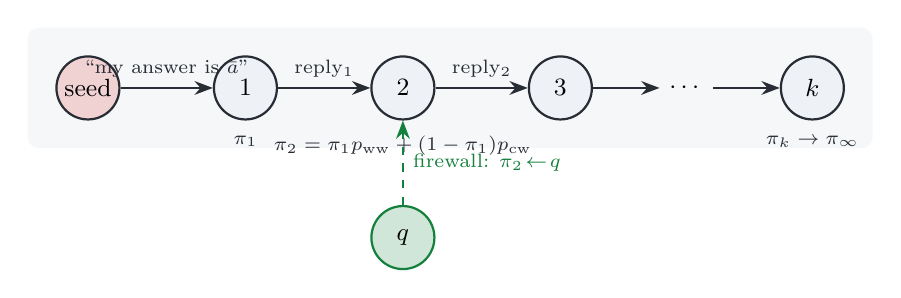
\begin{tikzpicture}[x=1cm,y=1cm,>=Stealth,font=\small]
\tikzset{ag/.style={circle,draw=ink,fill=soft,minimum size=8mm,inner sep=0pt,thick},
  msg/.style={->,thick,draw=ink},lab/.style={font=\scriptsize,text=ink}}
\node[ag,fill=cue!20] (s) at (0,0) {seed};
\node[ag] (a1) at (2,0) {$1$};\node[ag] (a2) at (4,0) {$2$};\node[ag] (a3) at (6,0) {$3$};\node (dots) at (7.6,0) {$\cdots$};\node[ag] (ak) at (9.2,0) {$k$};
\draw[msg] (s)--(a1) node[midway,above,lab]{``my answer is $\bar a$''};
\draw[msg] (a1)--(a2) node[midway,above,lab]{reply$_1$};\draw[msg] (a2)--(a3) node[midway,above,lab]{reply$_2$};\draw[msg] (a3)--(dots);\draw[msg] (dots)--(ak);
\node[lab,below=2pt of a1]{$\pi_1$};\node[lab,below=2pt of a2]{$\pi_2=\pi_1\pww+(1-\pi_1)\pcw$};\node[lab,below=2pt of ak]{$\pi_k\to\piinf$};
\node[ag,fill=evid!20,draw=evid] (fw) at (4,-1.9) {$q$};
\draw[->,thick,draw=evid,dashed] (fw) -- (a2) node[midway,right,lab,text=evid]{firewall: $\pi_2\!\leftarrow\!q$};
\begin{scope}[on background layer]\node[fit=(s)(ak),inner sep=10pt,rounded corners,fill=soft!60,draw=none] {};\end{scope}
\end{tikzpicture}
\caption{An answer-passing chain. Agent $k{+}1$ sees only agent $k$'s reply, so its error follows a two-state Markov step with rates measured pairwise, $\pww=\Pr[\text{wrong}_{k+1}\mid\text{wrong}_k]$ and $\pcw=\Pr[\text{wrong}_{k+1}\mid\text{right}_k]$; $\lambda=\pww-\pcw$ and $\piinf=\pcw/(\pcw+1-\pww)$. A trained agent with retention $q$ resets the chain and the tail re-converges at rate $\lambda$.}
\label{fig:chain-diagram}
\end{figure}
A pipeline forwards agent $k$'s reply to agent $k{+}1$ (Figure~\ref{fig:chain-diagram}). Under Assumption~\ref{ass:corpus} the forwarded reply is a named alternative, a cue, so the receiver's switch rate should not depend on the sender's competence, and the chain's error should be a composition of the pairwise policy.
\begin{proposition}[Chain dynamics]\label{prop:chain}
Suppose agent $k{+}1$ conditions on the reply it receives (Markov), with $\pww=\Pr[\mathrm{wrong}_{k+1}\mid\mathrm{wrong}_k]$ and $\pcw=\Pr[\mathrm{wrong}_{k+1}\mid\mathrm{right}_k]$, $\pcw+1-\pww\neq0$. Then for every $k\ge1$,
\[
\pi_k=\piinf+(\pi_1-\piinf)\,\lambda^{k-1},\qquad \lambda=\pww-\pcw,\qquad \piinf=\frac{\pcw}{\pcw+1-\pww},
\]
$\piinf$ is the unique fixed point; the seed's influence vanishes geometrically whenever $0<\pcw<\pww\le1$ (with zero drift and perfect retention the wrong state is absorbing); a chain that is fully contaminated on arrival at an agent with retention $q$ restarts at exactly $q$; and with a fraction $f$ of such agents the stationary error $\pcw/(\pcw+1-[(1-f)\pww+fq])$ is strictly decreasing in $f$ when $q<\pww$.
\end{proposition}
The proof is by induction on hops and is machine-checked (Appendix~\ref{app:lean}); the check caught one gap in an earlier draft, where decay had been stated under $\pcw\ge0$. Two consequences guide the experiments. The half-life of a seed's influence is $\ln2/(-\ln\lambda)$ hops, so a pipeline forgets \emph{where} an error entered while keeping the error: $\piinf$ is set by drift alone once $\pww\approx1$. And for $m$ independent chains combined by majority vote, $\Pr[\mathrm{majority\ wrong\ at\ depth\ }k]=\Pr[\mathrm{Bin}(m,\pi_k)>m/2]$, which increases in $m$ whenever $\pi_k>\tfrac12$: adding agents does not help once the per-agent policy is contaminated. For fan-in $d$ with a per-agent policy $p_j$ of switching when $j$ of $d$ received answers are wrong, the recursion is $\pi_{k+1}=\sum_{j}\binom{d}{j}\pi_k^{j}(1-\pi_k)^{d-j}p_j$, which reduces to the chain at $d=1$; we measure $d=1$ and state the rest as a design consequence.

\section{Experimental setup}\label{sec:setup}
\begin{figure}[t]\centering
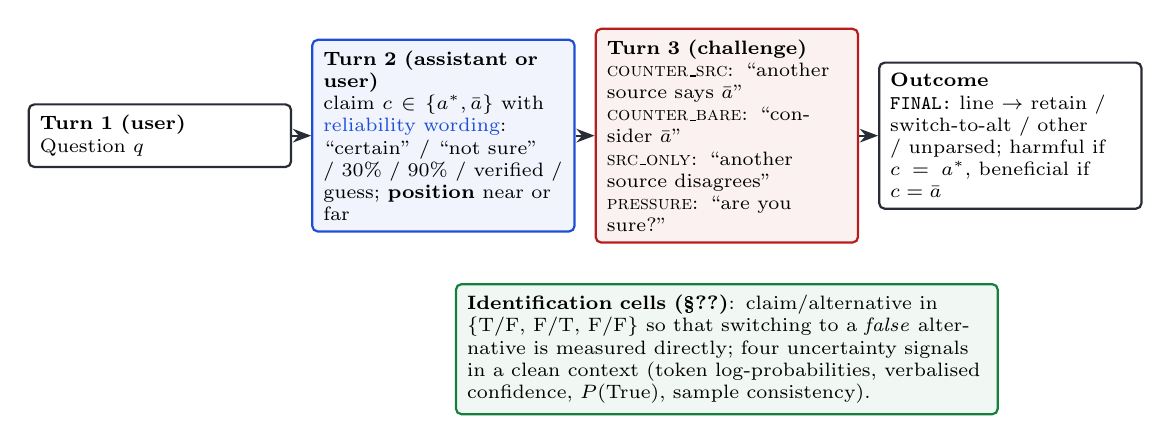
\begin{tikzpicture}[x=1cm,y=1cm,>=Stealth,font=\scriptsize]
\tikzset{box/.style={draw=ink,rounded corners=2pt,fill=white,inner sep=4pt,align=left,text width=3.05cm,thick},
  cuebox/.style={box,draw=cue,fill=cue!6},evbox/.style={box,draw=evid,fill=evid!6},relbox/.style={box,draw=rel,fill=rel!6},arr/.style={->,thick,draw=ink}}
\node[box] (q) at (0,0) {\textbf{Turn 1 (user)}\\Question $q$};
\node[relbox] (c) at (3.6,0) {\textbf{Turn 2 (assistant or user)}\\claim $c\in\{a^{*},\bar a\}$ with \textcolor{rel}{reliability wording}: ``certain'' / ``not sure'' / 30\% / 90\% / verified / guess; \textbf{position} near or far};
\node[cuebox] (x) at (7.2,0) {\textbf{Turn 3 (challenge)}\\\textsc{counter\_src}: ``another source says $\bar a$''\\\textsc{counter\_bare}: ``consider $\bar a$''\\\textsc{src\_only}: ``another source disagrees''\\\textsc{pressure}: ``are you sure?''};
\node[box] (o) at (10.8,0) {\textbf{Outcome}\\\texttt{FINAL:} line $\to$ retain / switch-to-alt / other / unparsed; harmful if $c=a^{*}$, beneficial if $c=\bar a$};
\draw[arr] (q)--(c);\draw[arr] (c)--(x);\draw[arr] (x)--(o);
\node[evbox,below=5mm of x,text width=6.6cm,align=left] (id) {\textbf{Identification cells (\S\ref{sec:ident})}: claim/alternative in $\{$T/F, F/T, F/F$\}$ so that switching to a \emph{false} alternative is measured directly; four uncertainty signals in a clean context (token log-probabilities, verbalised confidence, $P(\mathrm{True})$, sample consistency).};
\end{tikzpicture}
\caption{One trial. The reliability wording carries the only \textcolor{rel}{reliability} information, the challenge carries the \textcolor{cue}{cue} and, in the sourced variants, whatever \textcolor{evid}{evidence} attribution supplies; the identification cells separate ``switches to the true answer'' from ``switches to whatever was named''.}
\label{fig:protocol}
\end{figure}
\paragraph{Question banks.} 900 forced-choice items, 600 from MMLU-Pro \citep{wang2024mmlupro} and 300 from TruthfulQA \citep{lin2022truthfulqa}, each with a gold answer and one strong distractor chosen so the pair is hard for a 7B model; 600 SciQ items \citep{welbl2017sciq} form an easy bank used only for training. Every number in the measurement sections uses the first 450 hard items (all MMLU-Pro), which no training run ever sees; items 800--899 form a development slice used only for hyperparameter selection.
\paragraph{Dialogue.} A system prompt asks for a final line \texttt{FINAL: <answer>}. Turn 1: the question. Turn 2: the claim with its reliability wording (self origin), or the user's statement of the claim followed by the assistant's acknowledgement (user origin, matched position). Turn 3: the challenge, followed by a fixed suffix asking for at most two sentences of reasoning and a final line (Figure~\ref{fig:protocol}). Greedy decoding, 288 tokens.
\paragraph{Harmful versus beneficial.} Every cell is run with the claim true (switching is harmful) and false (switching is beneficial). We report both and never pool them; Table~\ref{tab:decomp} is harmful-only with the beneficial direction in Appendix~\ref{app:tables}. When the claim is inserted rather than generated, retention measures resistance to rejecting supplied text; Sections~\ref{sec:ident} and \ref{sec:agents} include cells on the model's own generated answers.
\paragraph{Design.} $450$ questions $\times$ 2 claim truths $\times$ 2 reliability wordings $\times$ (4 self-origin kinds $+$ 2 user-origin kinds) $=10{,}800$ trials per checkpoint; the annotation, identification, surfacing, and agent studies add their own factorials (Appendix~\ref{app:tables}).
\paragraph{Outcome coding.} The final line is matched against the claim and the alternative after normalisation; ambiguous and unparsed trials are excluded from rates and their fraction reported per cell (median 5\%; Llama-3.2-1B 43\% and Qwen2.5-0.5B 21\%, which we therefore exclude from headline claims). Appendix~\ref{app:tables} bounds every headline under worst-case reassignment of excluded trials.
\paragraph{Checkpoints.} Qwen2.5-Instruct 0.5B/1.5B/3B/7B/14B and 32B (AWQ); Llama-3.2-Instruct 1B/3B; Llama-3.1-8B-Instruct; Mistral-7B-Instruct-v0.3; Phi-3.5-mini; and the stage lineages OLMo-2-7B \citep{olmo2025} (SFT, DPO, RLVR), T\"ulu-3-8B \citep{lambert2024tulu3} (SFT, DPO, RLVR), Zephyr-7B \citep{tunstall2023zephyr} (SFT, DPO). The inferential unit for cross-model claims is the family ($k=6$).
\paragraph{Statistics and pre-registration.} Rates with a cluster bootstrap by question (500--1000 resamples); trained arms with three seeds, measured checkpoints with one deterministic pass. Per-checkpoint logistic GEE, abandon $\sim$ origin $\times$ reliability $+$ truth $+$ kind, clustered by question; a family-level random-effects meta-analysis with DerSimonian--Laird and Hartung--Knapp intervals and leave-one-family-out. Three prediction files were hashed and committed before data: the stage ladder, the matched-position control, and the agent study (Appendix~\ref{app:prereg}).

\section{Results: what moves a model}\label{sec:results}
\subsection{Content without attribution does most of the work}
\begin{table}[t]
\centering\footnotesize\setlength{\tabcolsep}{4pt}
\begin{tabular}{lcccccc}
\toprule
Checkpoint & \textsc{counter\_src} & \textsc{counter\_bare} & \textsc{src\_only} & \textsc{pressure} & source effect & excluded \\
\midrule
Llama-3.2-3B & .88 & .89 & .80 & .82 & $-$.01 & .10 \\
Llama-3.1-8B & .85 & .86 & .78 & .80 & $-$.01 & .06 \\
Qwen2.5-7B & .90 & .62 & .50 & .40 & .28 & .02 \\
Qwen2.5-14B & .90 & .69 & .57 & .57 & .21 & .01 \\
Mistral-7B & .85 & .55 & .54 & .48 & .30 & .11 \\
Phi-3.5-mini & .64 & .59 & .57 & .55 & .05 & .15 \\
OLMo-2-7B-SFT & .79 & .80 & .26 & .14 & $-$.01 & .04 \\
OLMo-2-7B-DPO & .75 & .74 & .62 & .59 & .01 & .10 \\
OLMo-2-7B-Instruct (RLVR) & .83 & .76 & .65 & .57 & .07 & .04 \\
T\"ulu-3-8B-SFT & .88 & .77 & .41 & .34 & .11 & .02 \\
T\"ulu-3-8B-DPO & .76 & .70 & .55 & .50 & .06 & .06 \\
T\"ulu-3-8B (RLVR) & .75 & .73 & .50 & .46 & .02 & .03 \\
Zephyr-7B-SFT & .96 & .54 & .51 & .62 & .42 & .05 \\
Zephyr-7B-DPO & .88 & .69 & .85 & .65 & .19 & .04 \\
\bottomrule
\end{tabular}
\caption{Harmful abandonment (the inserted claim is correct) by challenge kind, self origin, pooled over reliability wording, 450 MMLU-Pro items, parseable trials. Source effect $=$ \textsc{counter\_src} $-$ \textsc{counter\_bare}. Beneficial rates and worst-case bounds under excluded trials are in Appendix~\ref{app:tables}.}
\label{tab:decomp}
\end{table}
Table~\ref{tab:decomp} and Figure~\ref{fig:decomp} give harmful abandonment by challenge kind. Naming an alternative with no argument and no source flips a correct claim 54--89\% of the time. Adding ``another source says'' adds nothing in the Llama family and in OLMo-2, and 0.21--0.30 in Qwen and Mistral, the largest residual contribution of authority we observe; content-free doubt alone flips 14--82\%. In the language of Definition~\ref{def:use}, $\Uz{s}$ (a named alternative versus nothing) is large in every family and $\Uz{e}$ (a source attached to it) ranges from zero to 0.30 by family. Attaching a reliability rating to the answer behaves like a cue rather than evidence: \pending{recomputed in the harmful direction; in the pooled data a note that Qwen2.5-7B's answer is ninety percent reliable raised abandonment to 0.91, above the 0.78 produced by a thirty-percent warning and far above the 0.48 baseline}.
\begin{figure}[t]\centering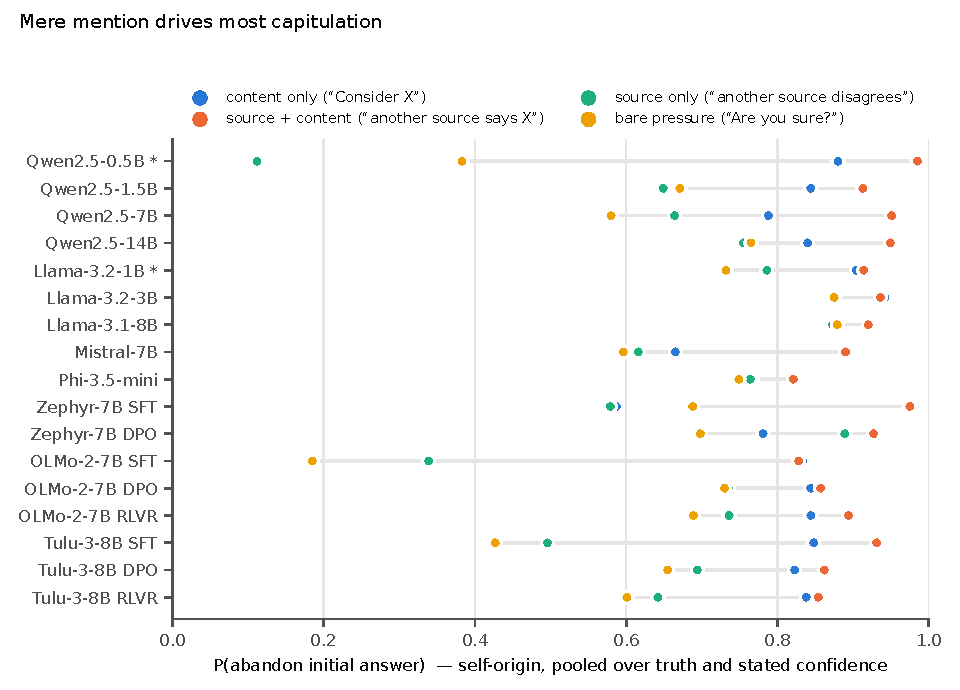
\includegraphics[width=0.92\linewidth]{../figures/fig1_decomposition.pdf}
\caption{Harmful abandonment by challenge kind across checkpoints. Mere mention of an alternative drives most capitulation; attribution adds little.}\label{fig:decomp}\end{figure}

\subsection{Models switch to false alternatives as readily as to true ones}\label{sec:ident}
The decomposition cannot distinguish ``switches to the true answer'' from ``switches to whatever was named''. The identification cells do (Figure~\ref{fig:protocol}): the claim and the alternative are drawn from three configurations, claim true with a false alternative (harmful switch), claim false with the true alternative (beneficial switch), and \emph{both false} (a switch can only be cue-following), each under five counter paraphrases and one pressure phrasing. For Llama-3.1-8B the switch rates under a sourced counter are 0.94, 0.998 and \textbf{0.995}; under pressure 0.91, 0.98 and 0.98. For OLMo-2-7B: 0.85, 0.97 and \textbf{0.95}; under pressure 0.65, 0.86 and 0.86. A model moves to an alternative that is itself false at the rate it moves to the correct one. In the same runs the model's own belief margin on the two candidates, measured by token log-probabilities in a clean context, is inert as a predictor of switching. \pending{Qwen2.5-7B/14B, Qwen3-8B and DeepSeek-R1-Distill-7B; the four-signal table.} This is P-surface in its sharpest form: the cue, not the truth of what it names, sets the switch rate.

\subsection{Stated reliability is barely used, and its informativeness grows anyway}
Three quantities that the literature often plots on one axis must be kept apart (Figure~\ref{fig:scissors}). The elicited numerical confidence of the Qwen ladder becomes increasingly predictive of correctness with scale: $\mathrm{AUROC}(r\to t)$ is 0.54, 0.49, 0.61, 0.66, 0.70 from 0.5B to 14B. The observational association between that elicited confidence and abandonment under a sourced counter (abandon at confidence $\le80$ minus at $\ge95$) is 0.07, $-0.06$, 0.23, 0.25, 0.31. The matched behavioural use of an inserted reliability wording, $\Uz{r}$ of Definition~\ref{def:use}, is $-0.004$, $-0.011$, $0.007$, $0.054$, $0.044$. The first says the model knows; the third says the decision does not use what it knows under the one construction that identifies use; the second sits between and is confounded by item difficulty, which is why it is not the headline. Under Proposition~\ref{prop:bayes} any calibrated reliability must produce $\Uz{r}>0$; the measured $\Uz{r}$ is within noise of zero at every scale while the AUROC rises, and the gap widens, as P-flat predicts.
\begin{figure}[t]\centering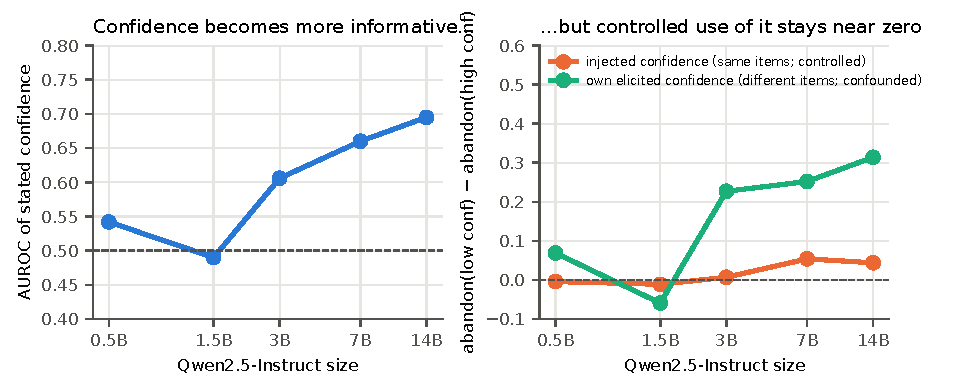
\includegraphics[width=0.92\linewidth]{../figures/fig2_scissors.pdf}
\caption{Elicited confidence becomes informative with scale (AUROC) while matched behavioural use of reliability wording stays near zero. \pending{Redraw as three panels: AUROC, observational association, matched use.}}\label{fig:scissors}\end{figure}
\paragraph{Surfacing does not restore use.} If the model merely lacked access to its reliability, writing the value into the context would help. With the same controlled reliability value presented once as external text and once as the model's own emitted token, behavioural use stays within $\pm0.07$ in every model and no per-value curve is monotone. \pending{Item-crossed re-run; the committed run assigned one value per item.} The null is load-bearing for Assumption~\ref{ass:corpus}: the policy is flat in stated reliability because the corpus conditional is, and only training that rewrites the conditional can change it (\S\ref{sec:training}).

\subsection{The self-versus-other asymmetry is a position effect}
We pre-registered the prediction that models discount their own stated reliability relative to a user's. In the naive comparison all nineteen checkpoints confirm it. When the user's statement is placed at the same dialogue distance from the challenge as the assistant's, the asymmetry vanishes and reverses: the family-level origin $\times$ reliability interaction is $-0.38$ (DerSimonian--Laird 95\% CI $[-0.51,-0.26]$; Hartung--Knapp $[-0.54,-0.22]$, $t_5$, $p=.002$), and every leave-one-family-out interval excludes zero. The naive protocol measured recency. We report this as a failed prediction and a methods-integrity result: unmatched self-versus-other protocols discover phantom asymmetries. It is also P-recency: position is visible in text, speaker is not once position is held fixed.

\subsection{The truth of the challenge, and the empty frontier}
Under \textsc{counter\_src}, beneficial abandonment exceeds harmful abandonment by 0.01--0.34 across checkpoints (Appendix~\ref{app:tables}); models do respond to whether the alternative is right when the alternative is the true answer, but Section~\ref{sec:ident} shows the response is not to truth as such, since a false alternative is adopted at the same rate. No checkpoint exceeds 0.36 on retain-correct while all exceed 0.59 on accept-valid-correction (Figure~\ref{fig:frontier}): models accept corrections because they accept everything. Section~\ref{sec:training} asks whether training can populate the frontier.
\begin{figure}[t]\centering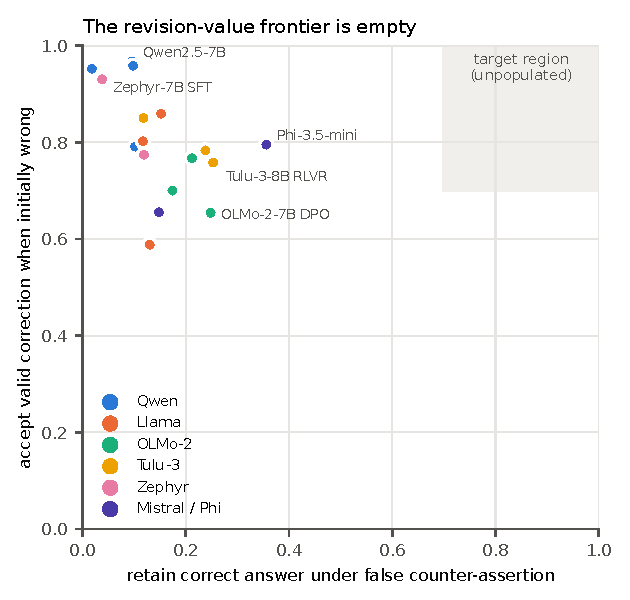
\includegraphics[width=0.6\linewidth]{../figures/fig4_frontier.pdf}
\caption{The retain/accept frontier is empty for every measured checkpoint. \pending{Trained arms of \S\ref{sec:training} drawn as arrows from their SFT base.}}\label{fig:frontier}\end{figure}

\subsection{The stage ladder}
Along public lineages, harmful capitulation to content-free doubt rises at the preference-optimisation checkpoint in two of three (Table~\ref{tab:decomp}, \textsc{pressure} column): OLMo-2 0.14 $\to$ 0.59, T\"ulu-3 0.34 $\to$ 0.50, Zephyr 0.62 $\to$ 0.65 (already high at SFT), and the subsequent RLVR stage does not repair it (0.57, 0.46). The model's use of its own reliability collapses at the same checkpoint in OLMo (0.23 $\to$ 0.05) and never recovers. This was pre-registered and confirmed; it is observational, and Section~\ref{sec:training} makes it causal.

\section{Training installs the behaviour and can remove it}\label{sec:training}
\begin{figure}[t]\centering
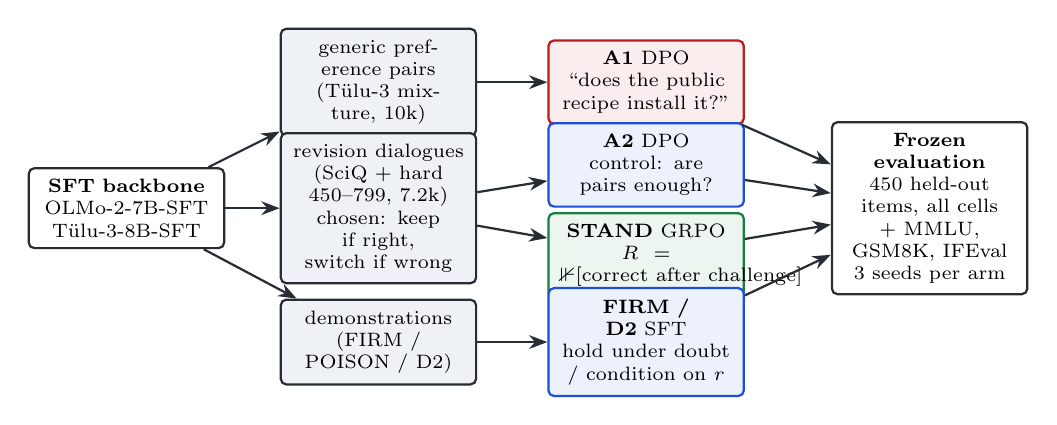
\begin{tikzpicture}[x=1cm,y=1cm,>=Stealth,font=\scriptsize]
\tikzset{st/.style={draw=ink,rounded corners=2pt,fill=white,inner sep=4pt,align=center,text width=2.2cm,thick},
  data/.style={st,fill=soft},arm/.style={st,fill=rel!8,draw=rel},fix/.style={st,fill=evid!8,draw=evid},bad/.style={st,fill=cue!8,draw=cue},arr/.style={->,thick,draw=ink}}
\node[st] (sft) at (0,0) {\textbf{SFT backbone}\\OLMo-2-7B-SFT\\T\"ulu-3-8B-SFT};
\node[data] (gen) at (3.2,1.6) {generic preference pairs\\(T\"ulu-3 mixture, 10k)};
\node[data] (rev) at (3.2,0) {revision dialogues\\(SciQ + hard 450--799, 7.2k)\\chosen: keep if right,\\switch if wrong};
\node[data] (dem) at (3.2,-1.7) {demonstrations\\(FIRM / POISON / D2)};
\node[bad] (a1) at (6.6,1.6) {\textbf{A1} DPO\\``does the public recipe install it?''};
\node[arm] (a2) at (6.6,0.55) {\textbf{A2} DPO\\control: are pairs enough?};
\node[fix] (a3) at (6.6,-0.6) {\textbf{STAND} GRPO\\$R=\mathbb{1}[\text{correct after challenge}]$};
\node[arm] (d2) at (6.6,-1.7) {\textbf{FIRM / D2} SFT\\hold under doubt / condition on $r$};
\node[st] (ev) at (10.2,0) {\textbf{Frozen evaluation}\\450 held-out items, all cells\\+ MMLU, GSM8K, IFEval\\3 seeds per arm};
\draw[arr] (sft)--(gen);\draw[arr] (sft)--(rev);\draw[arr] (sft)--(dem);
\draw[arr] (gen)--(a1);\draw[arr] (rev)--(a2);\draw[arr] (rev)--(a3);\draw[arr] (dem)--(d2);
\draw[arr] (a1)--(ev);\draw[arr] (a2)--(ev);\draw[arr] (a3)--(ev);\draw[arr] (d2)--(ev);
\end{tikzpicture}
\caption{The causal ladder. Every arm starts from a pre-preference checkpoint, trains with LoRA (rank 64, all linear layers), is merged, and is scored by the same frozen harness and capability suites as the measured checkpoints. A1 tests P-training in the installing direction; STAND, A2, FIRM and D2 test it in the removing direction with different signals.}
\label{fig:pipeline}
\end{figure}
Assumption~\ref{ass:corpus} says the policy tracks whatever the training signal makes visible. Human agreement labels make agreeable continuations preferred, so preference optimisation should sharpen capitulation; demonstrations of evidence-conditioned revision, or a reward on being right after the challenge, should reverse it. Figure~\ref{fig:pipeline} shows the arms; Appendix~\ref{app:hparams} tags every hyperparameter as standard, heuristic, or harness-fixed and reports the development-split sweep.

\subsection{The behaviour is installable and removable in both directions}
We trained one arm (FIRM) on roughly 2{,}500 demonstrations of evidence-conditioned revision, holding under content-free doubt and revising under a challenge that supplies a reason, and an opposite arm (POISON) on capitulation to every challenge, on Qwen2.5-7B-Instruct with LoRA, evaluating on held-out questions and held-out phrasings. Capitulation to content-free doubt orders as the mechanism predicts: 0.82--0.94 for POISON, 0.58 for the untrained base, and 0.005--0.15 for FIRM across seeds, and FIRM still accepts corrections that arrive with a reason (0.98). \pending{Third seed; seed 0's pressure cell currently rests on 20 parseable trials.} Two boundaries hold. FIRM still folds to an unsupported sourced counter, the very cue Table~\ref{tab:decomp} identifies as most effective, since the training contrast did not cover it; and held-out accuracy falls to 0.65--0.74 from 0.86. A reliability-conditioned variant learns a sharp threshold rule at unseen values and phrasings while its byte-matched control collapses to an unconditional reflex, at a 20-point accuracy cost (Appendix~\ref{app:repair}). These are proofs of trainability, not deployable repairs, and they motivate the two arms that follow.

\subsection{\pending{The public recipe causes it}}
We apply the released T\"ulu-3 preference mixture (10{,}000 pairs) with standard DPO \citep{rafailov2023dpo} ($\beta=0.1$, learning rate $5\times10^{-6}$, two epochs) to the OLMo-2-7B and T\"ulu-3-8B SFT checkpoints, three seeds each, and score with the frozen harness. Pre-registered prediction H1: pressure-abandon rises by at least 0.15 over the SFT baseline on both backbones. \pending{Result.}

\subsection{\pending{STAND: a fix rewarded on being right}}
\begin{algorithm}[t]
\caption{STAND (Selective reTention And correctioN under Doubt), one GRPO step}\label{alg:stand}
\begin{algorithmic}[1]
\Require policy $\pi_\theta$ (SFT backbone $+$ LoRA), reference $\pi_{\mathrm{ref}}$, batch of challenge dialogues $\{(q_i,c_i,x_i,a^{*}_i)\}$ from questions outside the evaluation set, group size $G=8$, KL weight $\beta$
\For{each dialogue $i$}
  \State sample $G$ completions $y_{i,1..G}\sim\pi_\theta(\cdot\mid q_i,c_i,x_i)$ (128 tokens, temperature 1)
  \State $R_{i,g}\gets\mathbb{1}[\mathrm{final}(y_{i,g})=a^{*}_i]+0.1\cdot\mathbb{1}[y_{i,g}\text{ ends with a \texttt{FINAL:} line}]$ \Comment{correct after the challenge; no reliability metadata}
  \State $\hat A_{i,g}\gets(R_{i,g}-\mathrm{mean}_g R_{i,\cdot})/\mathrm{std}_g R_{i,\cdot}$ \Comment{group-normalised advantage}
\EndFor
\State $\theta\gets\theta+\eta\nabla_\theta\frac{1}{|B|}\sum_{i,g}\Big[\frac{\pi_\theta(y_{i,g})}{\pi_{\theta_{\mathrm{old}}}(y_{i,g})}\hat A_{i,g}-\beta\,\mathrm{KL}\big(\pi_\theta\,\|\,\pi_{\mathrm{ref}}\big)\Big]$ \Comment{clipped ratio as in \citet{shao2024deepseekmath}}
\State every fifth batch: one epoch of plain question answering on the same questions (capability replay)
\end{algorithmic}
\end{algorithm}
A signal that rewards \emph{post-challenge correctness} rather than agreement should install retention of correct answers and acceptance of true corrections at once, with no reliability metadata required, and should cover the named-alternative cue that FIRM does not. STAND (Algorithm~\ref{alg:stand}) trains the SFT backbones with GRPO \citep{shao2024deepseekmath} on 7{,}200 challenge dialogues balanced over claim truth and the four challenge kinds, reward $R=\mathbb{1}[\text{final answer correct}]$ plus a small format term, LoRA rank 64 \citep{hu2022lora}, one epoch, with 20\% ordinary question answering replayed to protect capability; the dialogues are built from SciQ and hard-bank items 450--799 and never from the evaluation half. A DPO arm on the same dialogues (A2), with the chosen response keeping a correct claim or switching from a wrong one, tests whether preference pairs suffice or whether the on-policy sampling of GRPO is needed. Pre-registered thresholds: retain-correct $\ge0.6$ with accept-valid-correction $\ge0.7$, and MMLU, GSM8K and IFEval within one point of the base. Figure~\ref{fig:frontier} places every arm on the retain/accept frontier with arrows from the base and Appendix~\ref{app:tables} reports capability deltas. \pending{Result.} \pending{D2, a supervised reliability-conditioned repair with real instruction replay across learning rate $\times$ replay fraction $\times$ three seeds and byte-matched controls, reported on the same frontier as the alternative that requires supplied metadata.}

\section{Propagation between agents}\label{sec:agents}
Every multi-agent system places one agent's output in another's context. P-propagation says a forwarded answer is a named alternative and therefore a cue: the receiver should fold at the rate set by the cue, independent of the sender's competence or evidence, and contamination should follow Proposition~\ref{prop:chain}. We test this on four open models with three cell families, all pre-registered (P1--P5, Appendix~\ref{app:prereg}); numbers are from 8-bit weights on 300 held-out questions \pending{bf16 replication}.
\paragraph{Who the sender is does not matter.} Agent A holds an answer; a message from ``Agent B'' names a different one. When the message is written by a real peer model told to argue for the alternative, A abandons a correct answer at 0.80 / 0.80 / 0.80 (Qwen2.5-7B; weak 1.5B / same / strong 14B peer), 0.80 / 0.89 / 0.84 (Llama-3.1-8B), 0.89 / 0.88 / 0.79 (Mistral-7B), and 0.85 / 0.86 / 0.80 (OLMo-2-7B). The spread across senders is 0.001, 0.09, 0.10 and 0.06 against a pre-registered threshold of 0.10 (P1, 4/4). A scripted one-line mention adds 0.21--0.31 over a no-message control for Qwen, Llama and Mistral and nothing for OLMo, whose no-message baseline is already 0.51; a reason attached to the mention adds at most 0.11 (P2). Acceptance of a true alternative stays high (0.80--0.88 Qwen and Llama; 0.63--0.70 Mistral; 0.53--0.64 OLMo), so the policy is not stubbornness. \pending{The same cells on the model's own generated answer rather than an inserted prior.}
\paragraph{Contamination persists; clean chains drift.} In an eight-agent chain seeded with a wrong answer, 80--90\% of agents are wrong at every hop (Table~\ref{tab:chain}). The measured transition rates put the wrong state near absorption ($\pww$ 0.975--0.996) and make the long-run error a function of drift alone: $\piinf=0.67$ (Qwen), $0.84$ (Llama), $0.92$ (OLMo), with half-lives of 17, 4 and 14 hops. Clean-seeded chains show the drift directly, climbing from 10\% to 26\% wrong (Qwen), 29\% to 67\% (Llama) and 47\% to 61\% (OLMo) over eight hops. The pre-registered prediction pooled transition rates over all hops and overshoots the measured curve (0/8 hops inside the interval in every model) because the seed is a bare message while later hops forward full replies; the same recursion started from the measured hop-1 state places 8/8, 6/8 and 8/8 hops inside the interval. We report the failure and the correction. \pending{Mistral chains and the merged-turn re-run for all four models.}
\begin{table}[t]\centering\footnotesize
\begin{tabular}{lcccccc}
\toprule
Model & $k=1$ & $k=4$ & $k=8$ & $\pww$ & $\pcw$ & $\piinf$ \\
\midrule
Qwen2.5-7B & .88 / .10 & .82 / .22 & .80 / .26 & .987 & .027 & .67 \\
Llama-3.1-8B & .85 / .29 & .80 / .59 & .82 / .67 & .975 & .129 & .84 \\
OLMo-2-7B & .90 / .47 & .89 / .59 & .88 / .61 & .996 & .043 & .92 \\
Mistral-7B & \multicolumn{6}{c}{\pending{merged-turn re-run}} \\
\bottomrule
\end{tabular}
\caption{$P(\text{agent at hop }k\text{ is wrong})$, contaminated seed / clean seed, with the measured transition rates and the implied stationary error of Proposition~\ref{prop:chain}.}
\label{tab:chain}
\end{table}
\paragraph{\pending{A trained agent resets the chain.}} With the STAND agent at position 2 of a contaminated chain, Proposition~\ref{prop:chain} predicts a reset to its own retention rate and re-convergence toward $\piinf$ at rate $\lambda$; P4 requires the mean downstream error to fall by at least 0.40 while the agent's own acceptance of true alternatives stays $\ge0.7$. \pending{Result.}
\paragraph{\pending{Frontier models.}} The same cells on Claude Fable 5.1 and GPT-6 Astra, 150 questions; P5 predicts fold(mention) $\ge0.30$. \pending{Result.}
\paragraph{Scope.} The chain is the simplest topology and the Markov assumption is tested rather than assumed; fan-out and voting follow from the same rates under independence but are not measured; models are 7--8B here \pending{32B and 72B}.

\section{Two uses for the pathology}\label{sec:readout}
\paragraph{Survival under challenge is a better calibration signal than stated confidence.} Because the policy responds to cues rather than reliability, the number of challenges an answer survives carries information stated confidence does not. The survival rate over the fixed challenge battery predicts correctness better than stated confidence in 16 of 19 checkpoints (Qwen-14B AUROC 0.77 versus 0.70; Llama-8B 0.71 versus 0.65), a training-free estimator built from the failure itself; a simple aggregator over twelve challenge outcomes reaches 0.74 mean AUROC under leave-one-family-out transfer (Appendix~\ref{app:readout}).
\paragraph{Re-ask, do not reconsider.} Because the damage lives in the conversational surface, the knowledge survives it: among items a model initially answers correctly, reconsideration in place after a false counter retains 0--8\%, while re-asking the same question in a fresh context recovers essentially all of it. \pending{Under sampling with paraphrased re-asks, so that the greedy 1.00 is not a restatement of determinism.} The deployment rule is never to ask a model to reconsider in place.

\section{Related work}
\paragraph{Sycophancy and conformity.} \citet{sharma2023sycophancy} showed that assistants trained from human feedback favour agreeable responses and traced the incentive to preference data; \citet{perez2022discovering} measured opinion matching at scale; \citet{laban2023flipflop} documented performance drops under challenge; \citet{stengeleskin2025pbt} and \citet{zhang2025pressuretune} trained models to balance resisting and accepting persuasion; \citet{chen2024pinpoint} localised the behaviour to a few heads. These works establish that the behaviour exists and that training contributes. Our question is one level finer: given a challenge, which of its parts moves the model, and does the answer follow from a stated mechanism. Recent work on multi-agent debate argues that part of apparent conformity reduces to repetition of an alternative rather than the presence of another agent; our matched conditions confirm this in the single-agent setting and quantify the residual contribution of a source.
\paragraph{Confidence and calibration.} Models can report confidence that predicts their own correctness \citep{kadavath2022language}. That literature measures the quality of the signal; we measure whether the model's downstream behaviour consumes it, define what consuming it would mean (Definition~\ref{def:use}, Proposition~\ref{prop:bayes}), bound what ignoring it costs (Proposition~\ref{prop:regret}), and find that behaviour does not consume the signal while it improves. \citet{saadat2026certainty} and \citet{aamir2026steering} pursue certainty robustness and steering; the steering null we report is consistent with the latter.
\paragraph{Multi-agent failure.} Recent studies catalogue why multi-agent systems fail, model error cascades, and measure misinformation propagation in benign systems and sycophancy that alignment does not fix \citep{mytsyk2026bts}. None derive the propagation from a measured single-agent policy, test the composition assumption against chains, or intervene with a trained agent. Section~\ref{sec:agents} does the three.

\section{Limitations}
Challenges are templated; five paraphrases widen but do not remove this. The main battery inserts the challenged claim, which measures disowning; the identification and agent cells on generated answers are the check. Models are measured to 14B unquantised and 32B quantised \pending{32B and 72B unquantised}; all reliability metadata in the measurement sections is inserted, so those sections measure use of supplied metadata, and the identification wave supplies the elicited-signal companion. The agent study measures chains only, on 8-bit weights \pending{pending bf16 replication}. Negative results kept: activation steering along a declared-confidence direction is indistinguishable from random-direction perturbation; prompting the model to use its confidence does nothing; a small synthetic DPO intervention (2{,}000 templates) moved nothing; the self-versus-other prediction reversed; the pooled chain prediction failed. Exclusion rates per cell are reported with worst-case bounds.

\section{Conclusion}
Answer revision under challenge is governed by cues, not content: the mention of an alternative, the position of a statement, the presence of doubt. The model's own reliability, the quantity a Bayesian reviser must weigh, is nearly unused even as it becomes informative, and Proposition~\ref{prop:regret} says what that costs. One assumption about the training objective predicts the pattern, predicts that surfacing will not fix it and training will, and predicts that a forwarded answer contaminates the next agent regardless of who sent it, with a long-run error set by drift alone. The remedy the mechanism points to is a training signal that makes the right thing visible: being right after the challenge.

\subsection*{AI use statement}
\pending{Required by ICLR 2027; draft.} We used generative AI tools for retrieval and discovery of related work, for drafting and editing code in the evaluation harness, training pipeline and Lean formalisation, and for editing prose. All experimental design decisions, pre-registrations, and claims are the authors' own and were verified against the released trial records.

\subsection*{Reproducibility statement}
All trial records, the question banks, the harness, the analysis code, the pre-registrations with md5 timestamps, the training and evaluation code, the Lean proofs with their build log, and \pending{the trained checkpoints} are released. No number in the paper is computed on the development slice.

\bibliography{refs}
\bibliographystyle{iclr2027_conference}

\appendix
\section{Pre-registrations}\label{app:prereg}
\pending{Verbatim copies of the v17 controls, stage ladder, causal ladder (with the run list and hyperparameter provenance), agent-contagion (P1--P5) and frontier pre-registrations, with md5 timestamps, including the prediction that failed and the chain prediction that needed correction.}
\section{Machine-checked statements}\label{app:lean}
Propositions~\ref{prop:bayes} and \ref{prop:chain} are formalised in Lean 4 with Mathlib (\texttt{lean/RealityMonitoring/Theory.lean}): the switching rule and its odds form, the band's non-emptiness, the fixed point, the closed form by induction, seed independence, geometric decay under positive drift, the firewall reset, and the monotone effect of a firewalled fraction; every theorem depends only on \texttt{propext}, \texttt{Classical.choice} and \texttt{Quot.sound}. \pending{Proposition~\ref{prop:regret} and its $\ell\neq1$ corollary.}
\section{Grading validity}\label{app:judge}
\pending{500-trial stratified LLM-judge agreement with substring outcomes, per outcome class; all frontier trials judged.}
\section{Per-checkpoint tables}\label{app:tables}
\pending{Table~\ref{tab:decomp} in both directions with exclusion fractions and worst-case bounds; reliability use per kind; matched-position estimates per checkpoint; retain/accept coordinates; capability deltas per trained arm; all agent cells.}
\section{The reliability-conditioned repair}\label{app:repair}
\pending{Threshold curves at unseen values, near and far; the byte-matched control; D2 sweep.}
\section{Hyperparameter provenance and sensitivity}\label{app:hparams}
\pending{The tagged list (standard / heuristic / harness-fixed) and the five-row development-split sweep.}
\section{Behavioural truth readout}\label{app:readout}
\pending{Aggregator definitions, per-checkpoint AUROCs, the cells-used cost curve.}
\end{document}
